\documentclass[10pt]{beamer}

%PTBR
%\usepackage[brazilian]{babel}
\usepackage[utf8]{inputenc}
\usepackage[T1]{fontenc}
\usepackage{bm}
\usepackage{graphicx}
\usepackage[absolute,overlay]{textpos} %pacote para posicionar o logo na primeira página
%\usepackage[dvipsnames]{xcolor}

%\usepackage{enumitem}

\usetheme[progressbar=frametitle]{metropolis}
\usepackage{appendixnumberbeamer}

\usepackage{booktabs}
\usepackage[scale=2]{ccicons}

\usepackage{pgfplots}
\usepgfplotslibrary{dateplot}

\usepackage{xspace}
\newcommand{\themename}{\textbf{\textsc{metropolis}}\xspace}

\newcommand{\induceint}{\ensuremath{\Imc_{\Amc^{*}, \Tmc}}}
\newcommand{\fullminmod}{\ensuremath{\Imc_{\Amc^{*}, \Tmc}} \cup \Imc_{\min}(\Tmc)}

\usepackage{Macros}

%\definecolor{teal}{rgb}{0.0, 0.5, 0.5}
%\definecolor{darkorange}{rgb}{1.0, 0.55, 0.0}

\title{Lexicographic Closure and Typicality Models}

\titlegraphic{%
  \begin{picture}(0,0)
    \put(305,-120){\makebox(0,0)[rt]{
\includegraphics[width=6cm]{img/logos.png}}}
  \end{picture}}

\date{\today}
\author{Igor de Camargo e Souza Câmara}
\institute{University of São Paulo}

\begin{document}

\begin{frame}[plain]
  \titlepage
\end{frame}

\begin{frame}[fragile]{Motivation}
  \begin{quote}
    {\large
    ``At this time, we conjecture that \textbf{Lexicographic Closure} (...) can be similarly merged with our new semantics.'' \footnote{PENSEL, M. A Lightweight Defeasible Description Logic in Depth, 2019.}}
  \end{quote}
\end{frame}

\begin{frame}[fragile]{A simple DKB}
  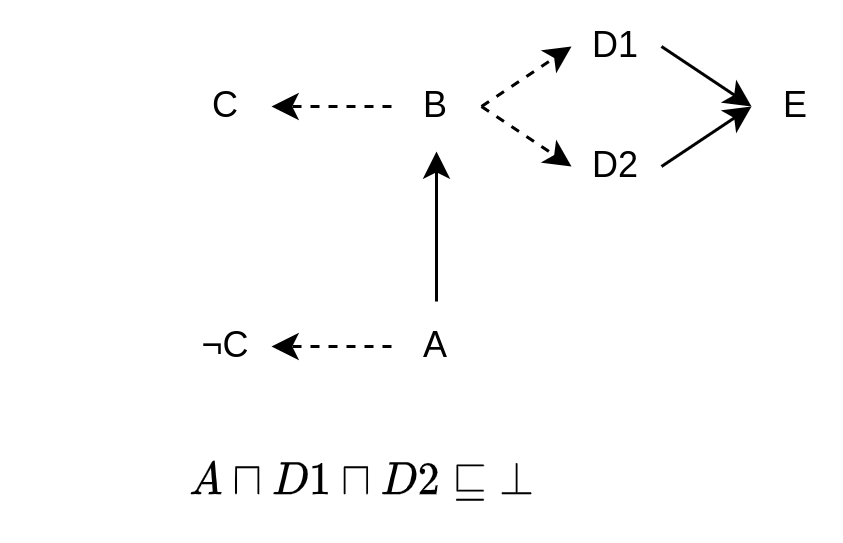
\includegraphics[scale=.35]{img/KB1.png}
\end{frame}

\begin{frame}[fragile]{Ranking the axioms and concepts}
  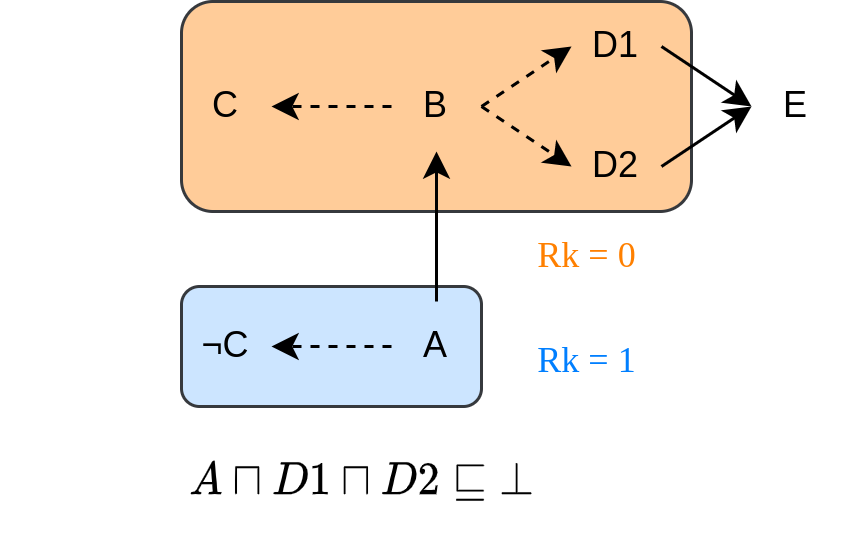
\includegraphics[scale=.35]{img/rank.png}
\end{frame}

\begin{frame}[fragile]{Rational Closure}
  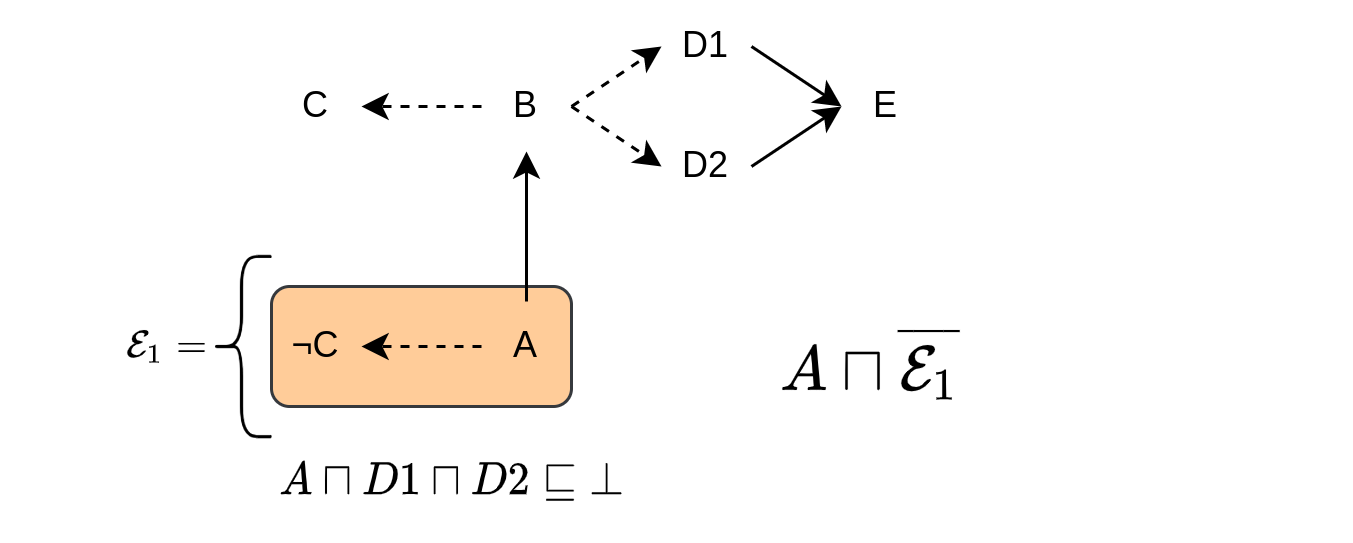
\includegraphics[scale=.3]{img/rationalc.png}
\end{frame}

\begin{frame}[fragile]{Lexicographic order}
\Large
$$\langle n_0, \dots, n_k \rangle <_{lex} \langle m_0, \dots, m_k \rangle$$

$$\textit{iff}$$

$$\exists i \in \{0, \dots, k\}.(\forall j < i.n_j = m_j) \land n_i < m_i$$
\end{frame}

\begin{frame}[fragile]{Lexicographic order -- Example}
  \Large
$$\langle 0, 0, 1 \rangle <_{lex} \langle 0, 1, 0 \rangle <_{lex} \langle 2, 0, 1 \rangle$$
\end{frame}

\begin{frame}[fragile]{Lexicographic rank \#1}
  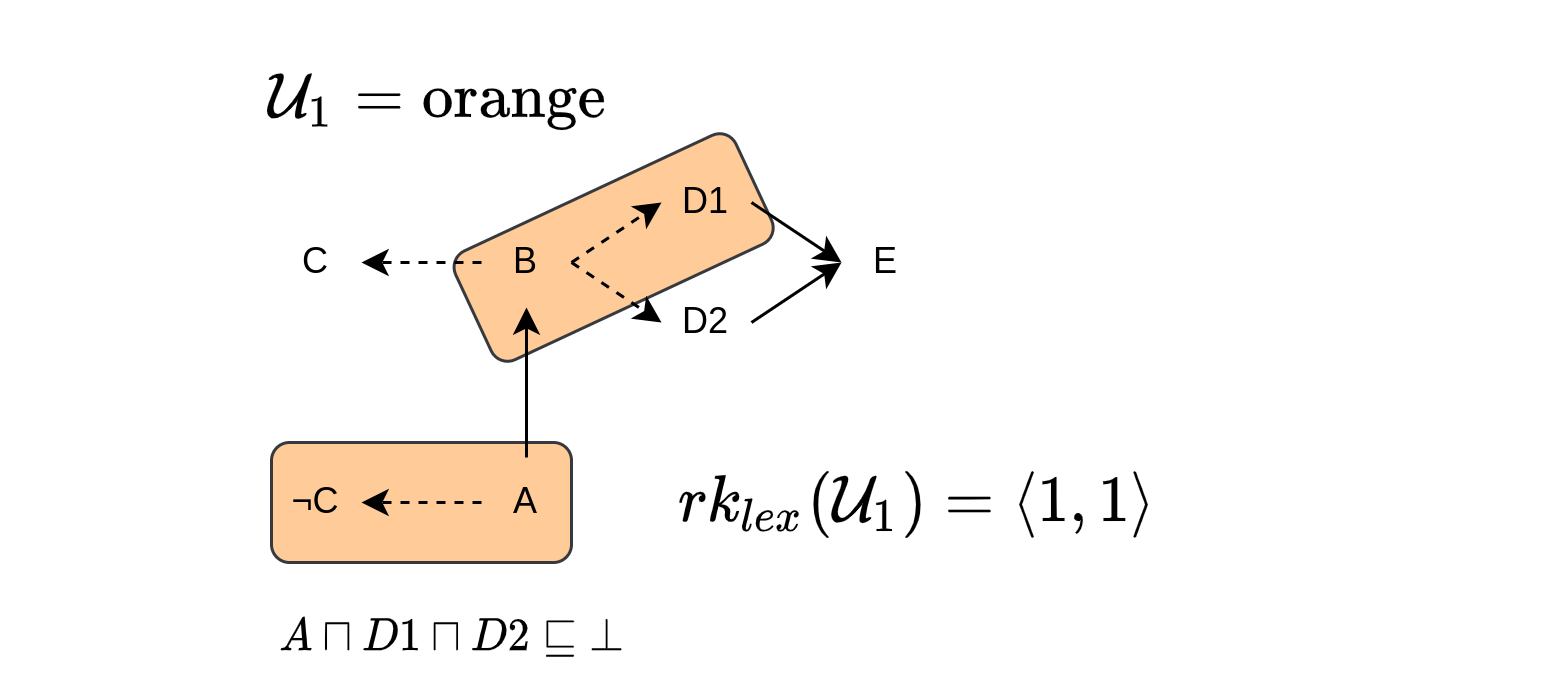
\includegraphics[scale=.27]{img/rklex1.png}
\end{frame}

\begin{frame}[fragile]{Lexicographic rank \#2}
  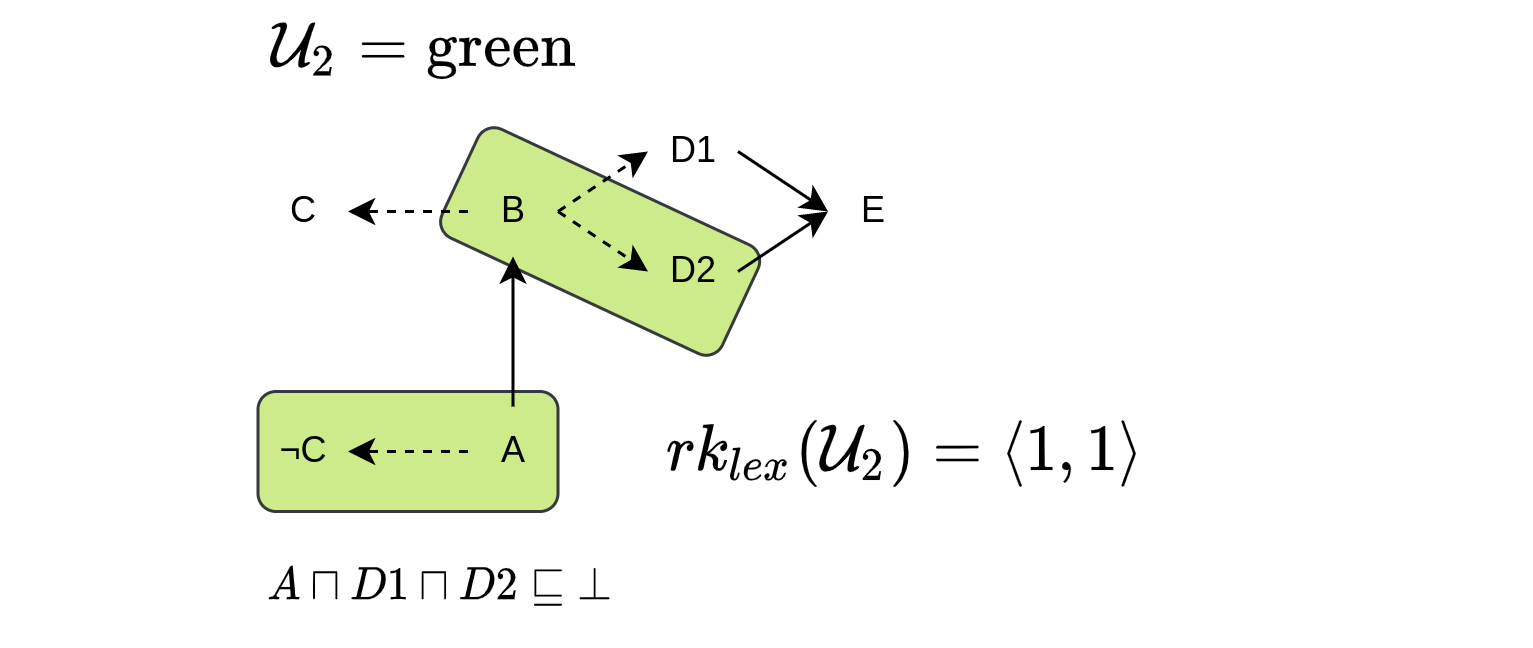
\includegraphics[scale=.27]{img/rklex2.png}
\end{frame}

\begin{frame}[fragile]{Lexicographic preference}

Lexicographic preference over $\Umc \subseteq \Dmc$ consistent with $A$

{\Large
$$\emptyset <_{lex} \Emc_0 <_{lex} \Umc_1 =_{lex} \Umc_2$$
}

\textit{i.e.}

{\Large
$$\langle 0, 0 \rangle <_{lex} \langle 1, 0 \rangle <_{lex} \langle 1, 1 \rangle =_{lex} \langle 1, 1 \rangle$$
}
\end{frame}

\begin{frame}[fragile]{Lexicographic Closure \#1 (Casini \& Straccia, 2012)}

  $\Kmc \models_{lex} C \definc D$ 
  
  iff 
  
  $\Kmc \models C \sqcap \overline{\Umc} \sqsubseteq D$, 
  
  for every $\Umc \subseteq \Dmc$ that 
  
  \begin{enumerate}
    \item Is not exceptional \textit{w.r.t.\xspace} $C$ and $\Kmc$.
    \item Is maximal according to the lexicographic order amongst the non-exceptionals.
  \end{enumerate} 

  \pause 

  \textbf{Example}

  $\Kmc \models_{lex} A \definc E$ 

  ${\color{orange}\Kmc \models A \sqcap \overline{\Umc_1} \sqsubseteq E}$ and ${\color{green}\Kmc \models A \sqcap \overline{\Umc_2} \sqsubseteq E}$

\end{frame}

\begin{frame}[fragile]{Lexicographic Closure \#2 (Pensel, 2019)}
  $\Kmc \models_{lex} C \definc D$ 
  
  iff 
  
  $\Kmc \models C \sqcap \overline{\Umc} \sqsubseteq D$, where
  \begin{align*}
    &\Umc_{lex} = \bigcap \{\Umc \subseteq \Dmc : \Umc \text{ is maximal amongst non-exceptional subsets} \\ 
    &\text{ of \Dmc w.r.t. \Kmc and } C\}
  \end{align*}

  \pause 

  \textbf{Example}

  $\Kmc \not \models_{lex} A \definc E$

  $\Umc_{lex} = \bigcap \{\Umc_1, \Umc_2\} = \{A \definc \lnot C\}$
  and
  $\Kmc \not\models A \sqcap \overline{\{A \definc \lnot C\}} \sqsubseteq E$
\end{frame}

\begin{frame}[fragile]{Preliminary Considerations}
  \begin{itemize}
    \item The characterization of lexicographic closure in Pensel (2019) does not match the one in Casini \& Straccia (2012). \pause 
    \item The multiple entailments in Casini \& Straccia (2012) adds a non-convex flavor by allowing the indirect expression of disjunctions (\eg $D_1 \sqcup D_2 \sqsubseteq E$) in the KB. \pause 
    \item It may be impossible to pinpoint a single $\Umc \subseteq \Dmc$ that could serve as the consistent subset to be materialized alongside the antecedent of a DCI, defining lexicographic closure. 
  \end{itemize}
\end{frame}

\begin{frame}[fragile]{Preliminary Considerations \# 2}
  \begin{itemize}
    \item The conjecture in Pensel (2019) remains open. \pause 
    \item Minimal typicality models can deal with this disjunctive falvor by having several maximal (w.r.t. lex rank) $\Umc \subseteq \Dmc$. \pause
    \item The resulting domain can have more than one more typical concept representative, and it represents LC multiple's entailments by each one of these elements.
  \end{itemize}
\end{frame}

\begin{frame}[fragile]{Lexicographic Domain -- example}
  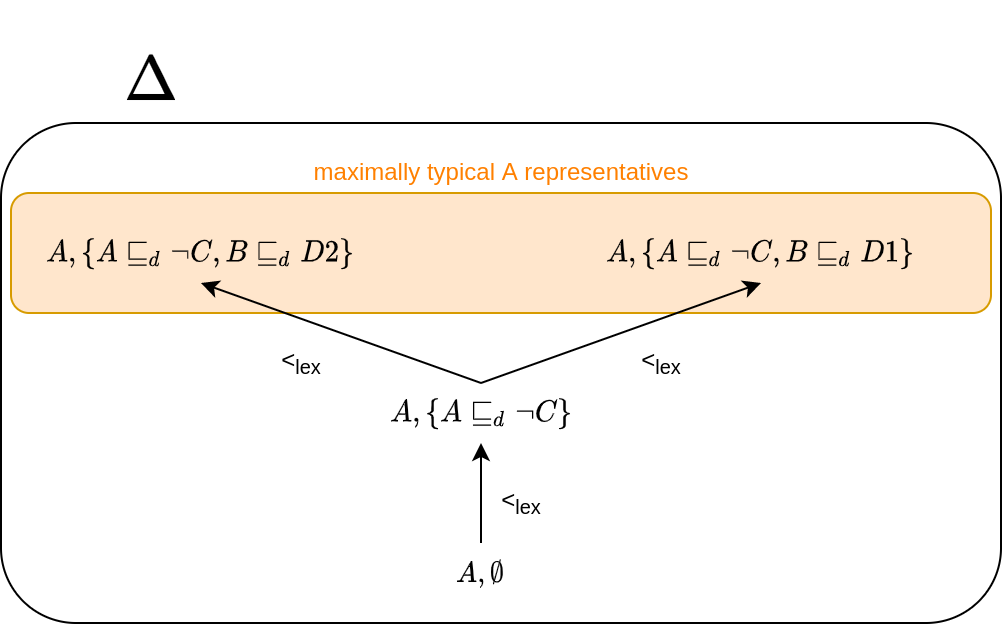
\includegraphics[scale=.32]{img/lexdomain.png}
\end{frame}

\begin{frame}[fragile]{Lexicographic Domain -- Definition}
  \begin{itemize}
    \item Let $Cons(\Kmc, C)$ return all the $\Umc \subseteq \Dmc$ non-exceptional w.r.t. $C$. \pause 
    \item Let $Cons^{lex}_{\max}(\Kmc, C)$ denote only the maximal (according to the lexicographic orders) elements of $Cons(\Kmc, C)$.
    \item To define $\Delta^{lex}$, for every $C$ in the relevant context, include every $\typel{C}{\Umc}$ s.t. $\Umc \subseteq \Umc'$ for some $\Umc' \in Cons^{lex}_{\max}(\Kmc, C)$.
  \end{itemize}
\end{frame}

% Old Last Slide

%\begin{frame}[fragile]{Preliminary Considerations \# 2}
%  \begin{itemize}
%    \item The conjecture in Pensel (2019) remains open, but the solution -- if there is any -- is not straightforward. \pause 
%    \item My intuition is that TM semantics cannot handle any kind of disjunctive knowledge, as it hurts the canonical model property. \pause
%    \item Alternative: build several minimal canonical models and take their intersection (to generate the minimal typicality model). \pause
%    \item Alternative 2: for the MTM, it does not matter. We can form the domain by including every maximal (w.r.t. lex rank) $\Umc \subseteq \Dmc$. There will be more than one maximal, but this is not a problem. \pause
%    \item The resulting domain can have more than one more typical concept representative, and it represents LC multiple's entailments by each one of these elements.
%  \end{itemize}
%\end{frame}

\end{document}




